\documentclass[english,man]{apa6}

\usepackage{amssymb,amsmath}
\usepackage{ifxetex,ifluatex}
\usepackage{fixltx2e} % provides \textsubscript
\ifnum 0\ifxetex 1\fi\ifluatex 1\fi=0 % if pdftex
  \usepackage[T1]{fontenc}
  \usepackage[utf8]{inputenc}
\else % if luatex or xelatex
  \ifxetex
    \usepackage{mathspec}
    \usepackage{xltxtra,xunicode}
  \else
    \usepackage{fontspec}
  \fi
  \defaultfontfeatures{Mapping=tex-text,Scale=MatchLowercase}
  \newcommand{\euro}{€}
\fi
% use upquote if available, for straight quotes in verbatim environments
\IfFileExists{upquote.sty}{\usepackage{upquote}}{}
% use microtype if available
\IfFileExists{microtype.sty}{\usepackage{microtype}}{}

% Table formatting
\usepackage{longtable, booktabs}
\usepackage{lscape}
% \usepackage[counterclockwise]{rotating}   % Landscape page setup for large tables
\usepackage{multirow}		% Table styling
\usepackage{tabularx}		% Control Column width
\usepackage[flushleft]{threeparttable}	% Allows for three part tables with a specified notes section
\usepackage{threeparttablex}            % Lets threeparttable work with longtable

% Create new environments so endfloat can handle them
% \newenvironment{ltable}
%   {\begin{landscape}\begin{center}\begin{threeparttable}}
%   {\end{threeparttable}\end{center}\end{landscape}}

\newenvironment{lltable}
  {\begin{landscape}\begin{center}\begin{ThreePartTable}}
  {\end{ThreePartTable}\end{center}\end{landscape}}

  \usepackage{ifthen} % Only add declarations when endfloat package is loaded
  \ifthenelse{\equal{\string man}{\string man}}{%
   \DeclareDelayedFloatFlavor{ThreePartTable}{table} % Make endfloat play with longtable
   % \DeclareDelayedFloatFlavor{ltable}{table} % Make endfloat play with lscape
   \DeclareDelayedFloatFlavor{lltable}{table} % Make endfloat play with lscape & longtable
  }{}%



% The following enables adjusting longtable caption width to table width
% Solution found at http://golatex.de/longtable-mit-caption-so-breit-wie-die-tabelle-t15767.html
\makeatletter
\newcommand\LastLTentrywidth{1em}
\newlength\longtablewidth
\setlength{\longtablewidth}{1in}
\newcommand\getlongtablewidth{%
 \begingroup
  \ifcsname LT@\roman{LT@tables}\endcsname
  \global\longtablewidth=0pt
  \renewcommand\LT@entry[2]{\global\advance\longtablewidth by ##2\relax\gdef\LastLTentrywidth{##2}}%
  \@nameuse{LT@\roman{LT@tables}}%
  \fi
\endgroup}


  \usepackage{graphicx}
  \makeatletter
  \def\maxwidth{\ifdim\Gin@nat@width>\linewidth\linewidth\else\Gin@nat@width\fi}
  \def\maxheight{\ifdim\Gin@nat@height>\textheight\textheight\else\Gin@nat@height\fi}
  \makeatother
  % Scale images if necessary, so that they will not overflow the page
  % margins by default, and it is still possible to overwrite the defaults
  % using explicit options in \includegraphics[width, height, ...]{}
  \setkeys{Gin}{width=\maxwidth,height=\maxheight,keepaspectratio}
\ifxetex
  \usepackage[setpagesize=false, % page size defined by xetex
              unicode=false, % unicode breaks when used with xetex
              xetex]{hyperref}
\else
  \usepackage[unicode=true]{hyperref}
\fi
\hypersetup{breaklinks=true,
            pdfauthor={},
            pdftitle={Children's social information gathering reflects sensitivity to uncertainty},
            colorlinks=true,
            citecolor=blue,
            urlcolor=blue,
            linkcolor=black,
            pdfborder={0 0 0}}
\urlstyle{same}  % don't use monospace font for urls

\setlength{\parindent}{0pt}
%\setlength{\parskip}{0pt plus 0pt minus 0pt}

\setlength{\emergencystretch}{3em}  % prevent overfull lines

\ifxetex
  \usepackage{polyglossia}
  \setmainlanguage{}
\else
  \usepackage[english]{babel}
\fi

% Manuscript styling
\captionsetup{font=singlespacing,justification=justified}
\usepackage{csquotes}
\usepackage{upgreek}



\usepackage{tikz} % Variable definition to generate author note

% fix for \tightlist problem in pandoc 1.14
\providecommand{\tightlist}{%
  \setlength{\itemsep}{0pt}\setlength{\parskip}{0pt}}

% Essential manuscript parts
  \title{Children's social information gathering reflects sensitivity to
uncertainty}

  \shorttitle{Information gathering reflects uncertainty}


  \author{Emily Hembacher\textsuperscript{1}, Benjamin deMayo\textsuperscript{1}, \& Michael C. Frank\textsuperscript{1}}

  \def\affdep{{"", "", ""}}%
  \def\affcity{{"", "", ""}}%

  \affiliation{
    \vspace{0.5cm}
          \textsuperscript{1} Stanford University  }

 % If no author_note is defined give only author information if available
      \newcounter{author}
                              \authornote{
            Correspondence concerning this article should be addressed to Emily Hembacher, 450 Serra Mall, Stanford, CA, 94305. E-mail: \href{mailto:ehembach@stanford.edu}{\nolinkurl{ehembach@stanford.edu}}
          }
                                                

  \abstract{We examined children's spontaneous information gathering in response to
lexical uncertainty. Children ages 2-5 (n=160) identified the referents
of familiar and novel labels. Referential ambiguity was manipulated
through the number of objects present and their familiarity (Experiments
1 and 2), and the availability of referential gaze (Experiment 2). In
both experiments, children sought disambiguating social information more
often while responding when the referent was ambiguous. In Experiment 2,
3- to 4-year-olds also demonstrated sensitivity to graded referential
evidence. These results suggest that social information gathering is an
active learning behavior that could contribute to language acquisition
in early childhood.}
  \keywords{information gathering; help seeking; word learning; uncertainty. \\

    \indent Word count: X
  }





\usepackage{amsthm}
\newtheorem{theorem}{Theorem}
\newtheorem{lemma}{Lemma}
\theoremstyle{definition}
\newtheorem{definition}{Definition}
\newtheorem{corollary}{Corollary}
\newtheorem{proposition}{Proposition}
\theoremstyle{definition}
\newtheorem{example}{Example}
\theoremstyle{definition}
\newtheorem{exercise}{Exercise}
\theoremstyle{remark}
\newtheorem*{remark}{Remark}
\newtheorem*{solution}{Solution}
\begin{document}

\maketitle

\setcounter{secnumdepth}{0}



Early childhood is marked by the rapid acquisition of new concepts,
rules, and language, and theories of cognitive development have
increasingly focused on the active role that children play in these
cognitive achievements (F. Xu \& Kushnir, 2013). Recent work highlights
that young children actively explore (Schulz \& Bonawitz, 2007) and ask
questions (Chouinard, Harris, \& Maratsos, 2007; Ruggeri, Sim, \& Xu,
2017) in ways that seem specifically targeted to reduce uncertainty.
Furthermore, they benefit from the ability to control the timing and
content of their learning (Markant, Ruggeri, Gureckis, \& Xu, 2016).

This burgeoning literature suggests that in many contexts children are
able to identify gaps in knowledge and act intentionally to fill those
gaps. However, it is still unclear how the reciprocal processes of
uncertainty monitoring and information gathering operate across
different learning domains and across development. Although the ability
to monitor epistemic uncertainty is logically prerequisite to active
learning, evidence about young children's metacognitive abilities has
been mixed and appears task-dependent. While some learning domains have
been studied repeatedly from an active-learning perspective (e.g.,
memory; {[}refs{]} causal learning {[}refs{]}), others have been
relatively ignored. In particular, we know little about children's
monitoring of lexical uncertainty and corresponding active learning
behaviors.

Awareness of lexical uncertainty or ignorance could be an important
mechanism for language acquisition. Knowing that you have incomplete
linguistic information (e.g., realizing that a word is unfamiliar or
that you can't retrieve the label for an object or concept) could prompt
active learning behaviors including asking for help or seeking other
disambiguating referential information. However, there is still limited
evidence about young children's tracking of lexical ambiguity or
associated active learning behaviors. In the following section we review
previous evidence about linguistic uncertainty monitoring and about
uncertainty monitoring in other domains.

\subsection{Development of uncertainty
monitoring}\label{development-of-uncertainty-monitoring}

A few previous studies have investigated children's awareness of lexical
uncertainty. One study examined whether 2-year-olds could report on
their own lexical ignorance when presented with unfamiliar words or
objects (Marazita and Merriman (2004)). They found that 2.5-year-olds
were better than chance at reporting that they did not know the name for
an unfamiliar item when asked, but still reported that they knew the
label \#\#\% of the time. When presented with nonsense words in a story,
they reported that they know what the word meant \#\#\% of the time.
Research in the selective trust literature has shown that children are
less willing to accept a new label for an unfamiliar object from a
previously inaccurate informant compared to an accurate one, suggesting
that young children do not treat all incoming linguistic input equally.
describe lyons2011 In one study, 3- to 5-year-olds used a pictorial
confidence scale to report on their certainty in their responses in
perceptual discrimination and lexical identification tasks (Lyons \&
Ghetti, 2011). Preschoolers reported being less confident when they
responded incorrectly, suggesting that they were aware of their
likelihood of accuracy based on their epistemic states.

Other studies have investigated the development of uncertainty
monitoring during early childhood in non-linguistic domains. Overall,
when asked explicitly about their confidence or knowledge, young
children tend to overestimate their likely accuracy and fail to
recognize their own ignorance. Hembacher and Ghetti (2014) (2014)
investigated children's confidence in their memories for pictures they
had studied using a pictorial confidence scale similar to Lyons et al.
They found that 3-year-olds were equally confident for correct and
incorrect answers, while 4- and 5-year-olds were more confident for
their correct answers (Hembacher \& Ghetti, 2014). Furthermore, only
5-year-olds were most confident about their memories for images they had
studied for longer. This is in contrast to Lyons et al. and Coughlin,
Hembacher, Lyons and Ghetti (2014) (2014) who found that even
3-year-olds were less confident for their incorrect responses in
perceptual and lexical tasks, although there were developmental
improvements across the age span tested. Thus, children's uncertainty
monitoring may depend on the cognitive task being reflected on.

Another series of studies has demonstrated children's failures to
recognize their ignorance or comprehension failures. Markman (1977) gave
preschoolers incomplete instructions to complete a task (i.e., a card
game or a magic trick), and asked them if they knew how to proceed. Even
after multiple prompts (e.g., \enquote{What do you think?}, \enquote{Do
you have any questions?}), children did not indicate that they were
unsure how to play the game. On average, 1st graders did not ask any
questions until they were asked \enquote{Can you tell me how to play?},
which presumably forced them to confront their ignorance of the critical
steps. Children also report knowing the unseen contents of a box if they
have seen several items that may have gone into the box (i.e., they have
\enquote{partial exposure} to the contents) until the age of 6 (Rohwer,
Kloo, \& Perner, 2012).

In sum, there is mixed evidence about young children's metacognitive
competencies in tasks that require explicit responses from children.
However, these paradigms may underestimate children's ability to track
epistemic uncertainty and act on it. One possibility is that children's
tracking of uncertainty is apparent in their spontaneous
information-seeking behaviors before they can report on it explicitly.
In the following section we review evidence that young children who fail
explicit metacognitive tasks nonetheless explore and seek information
selectively based on uncertainty.

\subsection{Development of Spontaneous
Information-seeking}\label{development-of-spontaneous-information-seeking}

First, a collection of studies have taken inspiration from comparative
metacognition research and asked whether children's spontaneous
information-seeking behaviors track uncertainty. For example, Call and
Carpenter (2001) had 2-year-olds choose between several tubes to find a
hidden sticker. They found that the toddlers were more likely to peek
inside a tube before choosing when they had not seen the baiting of the
tubes compared to when they had, suggesting they were aware of their
knowledge or ignorance and selectively sought confirmatory evidence
before committing to a response when they did not know a sticker's
location.

Other studies have shown that young children can opt out of responding
or seek help when uncertain of their memories. Balcomb and Gerken (2008)
had 3.5-year-olds complete a memory task in which they could opt out of
responding to individual trials. Children performed worse on trials they
had opted out of when they were forced to answer them later on,
suggesting that they used the opt-out option strategically to avoid
answering when they were uncertain about their responses. In another
study, Goupil, Romand-Monnier, and Kouider (2016) trained 20-month-olds
to look at their parents if they needed help with a memory task in which
they had to locate a hidden toy. Toddlers were more likely to seek help
when they were completely ignorant of the toy's location, and when the
task was more difficult because the delay between hiding and test was
longer. These studies suggest that young children can monitor the
strength (or absence) of memories and seek information when they are
less likely to respond correctly.

There is also evidence that young children selectively explore when
evidence is confounded (i.e., when existing evidence supports multiple
causal hypotheses). For example, Schulz \& Bonawitz (2007) found that
preschoolers spent more time playing with a toy when they witnessed
confounded evidence about its causal structure. Children who experienced
a demonstration of a toy in which two levers were simultaneously
depressed and caused two simultaneous events (a toy duck and puppet
popping up) spent more time playing with that toy compared to children
who saw a demonstration in which one lever was depressed at a time,
revealing the unique function of each lever. This finding is consistent
with the prediction that preschool-aged children track causal ambiguity
and spontaneously explore more when they do not have sufficient evidence
to isolate a cause for an effect.

Infants have also been shown to seek information selectively under
conditions of ambiguity, and explore or allocate attention to
information sources that are most likely to disambiguate. For example,
in one pair of studies, 7- and 8-month-olds attended longer to visual
displays (Kidd, Piantadosi, \& Aslin, 2012) or auditory stimuli (Kidd,
Piantadosi, \& Aslin, 2014) that were neither too complex nor too
simple, and thus afforded the greatest learning opportunity.
Twelve-month-old infants have also been shown to track the likelihood of
different events (e.g., a red ball exiting a container full of moving
red and blue balls) based on reasoning about multiple cues ---
numerosity (the number of red compared to blue balls), physical distance
(the distance from a red ball to the opening of the container) and time
(how long the scene was occluded before the ball left the container).
Intriguingly, infants' surprisal (looking time) tracked with uncertainty
about the likelihood of events --- for example, at intermediate
occlusion times, infants' looking time was graded with respect to
distance and numerosity in an additive fashion (Teglas et al., 2011).

\subsection{Current study}\label{current-study}

The present study investigates children's information-seeking behaviors
on the basis of lexical ambiguity. Specifically, we ask whether children
are more likely to seek disambiguating social information by looking at
the experimenter when they are uncertain of the referent of a label they
have been asked to act on. We chose to examine this ability in early
childhood (ages 2 to 5), because, as discussed, research under a
metacognitive framework has identified this as a developmental period in
which children improve substantially in their ability to identify their
own ignorance and uncertainty (Coughlin et al., 2014; Hembacher \&
Ghetti, 2014; Lyons \& Ghetti, 2011; Rohwer et al., 2012).

We manipulated lexical ambiguity by adapting a paradigm used by Vaish,
Demir and Baldwin (2011) (2011) to test infants' selective gaze
referencing. In that study, 12- to 18-month-olds heard an experimenter
produce a label for an object in the presence of one or two novel
objects. Infants looked at the experimenter more often when there were
two objects present, and the referent was thus ambiguous. This evidence
is interpreted as suggesting that older infants recognize the need for
disambiguating information, and reference the speaker's gaze direction
accordingly.

Here, we expand on this finding to ask whether 2- to 5-year-olds seek
social information throughout the course of a task in which a speaker
labels an object and asks the child to put the named object in a bucket.
Similar to Vaish et al., we examined the number of times children looked
up at the experimenter depending on the ambiguity of the label. We
examine children's use of social information during labeling, similar to
Vaish et al., but also during children's decision about which object to
place in the bucket. We also control for the number of objects by
including unambiguous trials with two familiar objects, one familiar
object, and one novel object, and the ambiguous trials with two novel
objects.

In Experiment 2, we additionally manipulate the amount of referential
evidence available allowing us to investigate whether preschoolers'
information-gathering is sensitive to graded lexical uncertainty (i.e.,
whether they are increasingly likely to answer independently without
seeking information as the amount of referential evidence increases).
There are several reasons to investigate children's sensitivity to
graded evidence. First, probabilistic models of cognition and learning
require that individuals be able to track the amount of evidence for
alternative beliefs (and corresponding uncertainty), perhaps through
heuristics such as \enquote{win-stay lose-sample} (Bonawitz, Denison,
Gopnik, \& Griffiths, 2014). If preschool-aged children do track
accumulating evidence as assumed by these models, their
information-gathering behaviors should be graded with respect to the
amount of evidence for a belief.

More generally, a complete theory of early metacognition and learning
should encompass children's ability to respond appropriately to graded
evidence. Metacognitive theories assume that effective behavioral
regulation and response selection rely on individuals' abilities to
track the likelihood of being correct based not only on complete
knowledge or ignorance, but on graded evidence (Lyons \& Zelazo, 2011).
For example, having more information in support of a belief should make
individuals more willing to share that information with others, and
having less information should motivate help-seeking (Ghetti, Hembacher,
\& Coughlin, 2013). In sum, the present study investigates whether
children ages 2 to 5 seek disambiguating social information on the basis
of lexical ambiguity. If so, this could be an important mechanism for
language acquisition during early childhood.

\begin{figure}
\centering
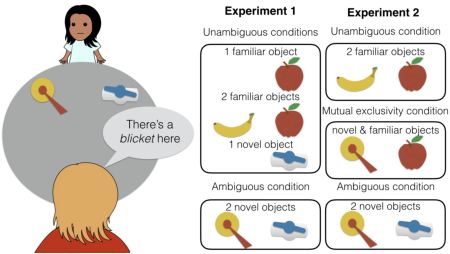
\includegraphics{figs/design-1.pdf}
\caption{\label{fig:design}Study design for Experiments 1 and 2. Children
were shown one or two objects, heard a label, and were asked to place
the labeled object in a bucket. Referential ambiguity was manipulated
through the familiarity of the objects present and through the
availability of referential gaze.}
\end{figure}

\section{Experiment 1}\label{experiment-1}

In Experiment 1, we examined whether children would visually reference a
speaker more often when the speaker produced a referentially ambiguous
label compared to an unambiguous label. Children sat across from an
experimenter who labeled an object on the table between them (Figure
\ref{fig:design}). The experimenter then asked the child to place the
named object in a bucket. Across trials, there were either one or two
objects on the table, which were either familiar or novel to the child.
This design allowed us to test whether merely having more than one
object present is sufficient to increase information gathering, or if
referential ambiguity (and thus epistemic uncertainty) is the underlying
factor. If the latter is true, we expected children to increase their
looking to the experimenter only on trials with two unfamiliar objects,
when the object-label mapping was not known and could not be inferred.

We were interested in the amount of information gathering children
exhibited across the trial. We considered four different phases of each
trial based on the notion that children might expect different social
information at different stages of the task. Specifically, we predicted
that children might expect the speaker's gaze direction to be
informative during the labeling itself, as speakers tend to look at
objects they refer to. We also predicted that later in the trial, as
children reached for an object and placed it in the bucket, they might
expect evaluative feedback about their choice (e.g., facial expressions
of encouragement or discouragement).

\subsection{Methods}\label{methods}

\subsubsection{Participants}\label{participants}

We recruited a planned sample of 80 children ages 2-5 years from the
Children's Discovery Museum in San Jose, California\footnote{Planned
  sample size, exclusion criteria, and analysis plan preregistered at
  \url{https://osf.io/y7mvt}.}. The sample included 20 2-year-olds (mean
age 31.7 months), 20 3-year-olds (mean age 42.7 months), 20 4-year-olds
(mean age 55.8 months), and 20 5-year-olds (mean age 65.1 months). An
additional 20 children participated but were removed from analyses
because they heard English less than 75\% of the time at home (\emph{n}
= 10), because they were unable to complete at least half of the trials
in the task (\emph{n} = 4), because of parental interference (\emph{n} =
1), or due to experimenter or technical errors (\emph{n} = 5).

\subsubsection{Stimuli and Design}\label{stimuli-and-design}

Children were presented with one or two objects, heard a label, and were
asked to put the labeled object in a bucket. Half of the objects were
selected to be familiar to children (e.g., a cow) and half were selected
to be novel (e.g., an usual-looking nozzle). The familiar items had
names that the majority of children recognize by 24 months (Frank,
Braginsky, Yurovsky, \& Marchman, 2016). There were four possible trial
types based on the number and familiarity of the objects present: one
familiar object (F), one novel object (N), two familiar objects (FF),
and two novel objects (NN). There were three trials of each type, for a
total of twelve trials. Trial types were presented sequentially in an
order that was counterbalanced across participants. The assignment of
individual objects to trial types was counterbalanced. On F and FF
trials, the familiar label for the target object was used (e.g.,
\enquote{cow}). On N and NN trials, a novel label was used (e.g.,
\enquote{dawnoo}).

The critical manipulation was of referential ambiguity; F and FF trials
were referentially unambiguous, as children were expected to be certain
about the objects and their labels. Similarly, on N trials, children
were expected to be certain about the label referent as there was only
one option. However, NN trials were referentially ambiguous, as the
novel label could apply to either novel object.

Throughout the task, the experimenter never gazed at the object they
were labeling, or responded to children's verbal or non-verbal bids for
help by indicating the correct object. Thus, children were expected to
remain uncertain about the referent for the duration of the trial when
two novel objects were present.

\subsubsection{Procedure}\label{procedure}

Throughout the study, the child sat at one end of a large circular
table, and the experimenter stood at the opposite end. Each trial
proceeded as follows: the experimenter placed one or two objects on the
left and/or right sides of the table, out of reach of the child so that
the child could not interact with the toys during the labeling event.
For one-object trials, the location of the object (left or right)
alternated between trials. After placing the objects, the experimenter
said \enquote{Hey look, there's a (target) here.} The experimenter gazed
at the center of the table rather than the object they labeled. The
experimenter waited approximately two seconds based on a visual
metronome placed within view before saying, \enquote{Can you put the
(target) in the bucket?} They then pushed the object(s) forward within
reach of the child, and placed a plastic bucket in the center of the
table, also within reach of the child. If the child did not respond
within 10 seconds, the experimenter repeated the question. The
experimenter provided no accuracy feedback to children throughout the
trial. After the child placed an object in the bucket, the experimenter
said \enquote{okay!} or \enquote{thank you!} to maintain a positive
interaction without providing information about accuracy. Prior to the
twelve experimental trials, there were two training trials: an F trial
and an FF trial, to acquaint the child with the procedure. If children
chose the wrong object on the FF trial (which happened rarely), they
were corrected. A camera placed to the side of the experimenter captured
the participant's face, so that looking behavior could be coded from
video.

\subsubsection{Coding procedure and analytic
plan}\label{coding-procedure-and-analytic-plan}

Videos were coded using DataVyu software (\url{http://datavyu.org}). For
each participant, we coded the \emph{number of times} they referenced
the experimenter throughout each trial. An alternative analytic option
would be to simply code \emph{whether or not} children looked at the
experimenter. However, during piloting, we found that most children
looked up to the experimenter at least once while they were labeling the
object, suggesting that a binary measure of looking would not be
meaningful.

Because we were interested in the precise circumstances in which
children feel uncertain enough to reference a speaker, we coded the
number of looks that occurred during four distinct phases of the trial:
a \emph{label} phase, which began at the utterance of the label and
ended when the experimenter began to slide the objects, a \emph{slide}
phase, in which the experimenter slid the object(s) into the child's
reach, a \emph{planning} phase, which began at the end of the slide and
ended when the child touched an object, and a \emph{response} phase,
which began when the child touched an object and ended when the child
released the object into the bucket. If a look began in one phase but
continued into another, we counted it as a look in both phases.

We also noted any trials that should be excluded from analyses due to
the child's interference with the timing of the trial (e.g., talking
over the experimenter), experimenter error, or outside distractions that
interfered with the timing of the trial (e.g., noise from a sibling).
These trial-wise exclusion criteria were preregistered. In total, we
excluded 1.6\% of trials from 2-year-olds, 2.0\% of trials from
3-year-olds, 1.9\% of trials from 4-year-olds, and 2.0\% of trials from
5-year-olds on this basis. A second coder independently scored the
number of looks for one third of the trials for each participant to
establish reliability. Inter-rater reliability for the number of looks
in each phase was high, intraclass correlation \emph{r} = .97, \emph{p}
\textless{} .001.

Table \ref{tab:phases} displays the average durations of each of the
four phases. The \emph{label} and \emph{response} phases are longer on
average than the \emph{planning} and \emph{slide} phases. However, note
that we are interested in comparing the amount of looking across
ambiguity conditions and not across phases directly.

To quantify the effects of the number and familiarity of objects on
children's looking, along with any developmental trends, we planned to
fit a linear mixed-effects regression. Mixed-effects models account for
both fixed and random factors (such as participants and stimuli). As
such, they provide a more accurate estimate of whether results will
generalize beyond the participants and items that were sampled (Baayen,
Davidson, \& Bates, 2008). As recommended by Barr, Levy, Scheepers, and
Tily (2013) (2013), we begin with a maximal model and trim according to
our standard laboratory procedures\footnote{Standard laboratory analytic
  procedures available at \url{https://osf.io/zqzsu/wiki/home/}}:
\texttt{number\ of\ looks\ \textasciitilde{}\ number\ of\ objects\ *\ familiarity\ *\ phase\ *\ age\ in\ months\ +\ (number\ of\ objects\ *\ familiarity\ \textbar{}\ subject)\ +\ (1\ \textbar{}\ trial)}.
Random effects are denoted by parentheses. This model specification was
preregistered, as noted above.

\subsection{Results and Discussion}\label{results-and-discussion}

\subsubsection{Accuracy}\label{accuracy}

\begin{figure}
\centering
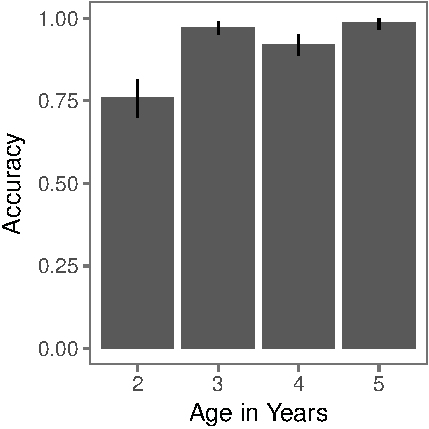
\includegraphics{figs/acce1-1.pdf}
\caption{\label{fig:acce1}Accuracy for FF trials in Experiment 1. Error bars
are 95 percent confidence intervals.}
\end{figure}

\begin{table}[b]
\centering
\begin{tabular}{llrr}
  \hline
Experiment & Phase & Mean Duration & SD \\ 
  \hline
1 & label & 5065 & 907 \\ 
  1 & slide & 870 & 194 \\ 
  1 & planning & 1270 & 2246 \\ 
  1 & response & 3632 & 4575 \\ 
   \hline
2 & label & 5239 & 748 \\ 
  2 & slide & 819 & 1307 \\ 
  2 & planning & 791 & 10327 \\ 
  2 & response & 4085 & 5032 \\ 
   \hline
\end{tabular}
\caption{Phase Durations (in ms)} 
\label{tab:phases}
\end{table}

We examined children's accuracy for those trials in which a correct
response was possible (i.e., FF trials). Children sometimes put two
items in the bucket (2-year-olds: 30.8\% of 2-object trials;
3-year-olds: 15.0\%; 4-year-olds: 7.5\%; 5-year-olds: 9.2\%), despite
instructions to choose only one. The first object children put in the
bucket was coded as their response. Children in each age group were
equally likely to put two objects in the bucket for familiar and
unfamiliar trials (2-year-olds: \emph{t}(19) = 0.53, \emph{p} =0.60;
3-year-olds: \emph{t}(19) = 1.45, \emph{p} =0.16; 4-year-olds:
\emph{t}(19) = -0.72, \emph{p} =0.48; 5-year-olds: \emph{t}(19) = 0.37,
\emph{p} =0.72), suggesting that they put two objects in the bucket
because it was a fun activity and difficult to inhibit, and not because
they did not know the referent. Among FF trials in which children placed
two items in the bucket, they put the correct item in first about half
of the time (8/19 trials total for 2-year-olds; 5/6 for 3-year-olds; 0/2
for 4-year-olds; 2/4 for 5-year-olds).

Children also occasionally declined to choose an item (0.4\% of trials);
these trials are excluded from accuracy analyses. Children's accuracy is
displayed in Figure \ref{fig:acce1}. Overall children generally chose
the correct item for FF trials, indicating that they understood the task
and were motivated to answer correctly. While 3- to 5-year-olds
performed close to ceiling (92\% - 99\%), 2-year-olds were less accurate
(76\%), but still performed significantly above chance (\emph{t}(19) =
23.0 , \emph{p} \textless{} .001).

\begin{figure}
\centering
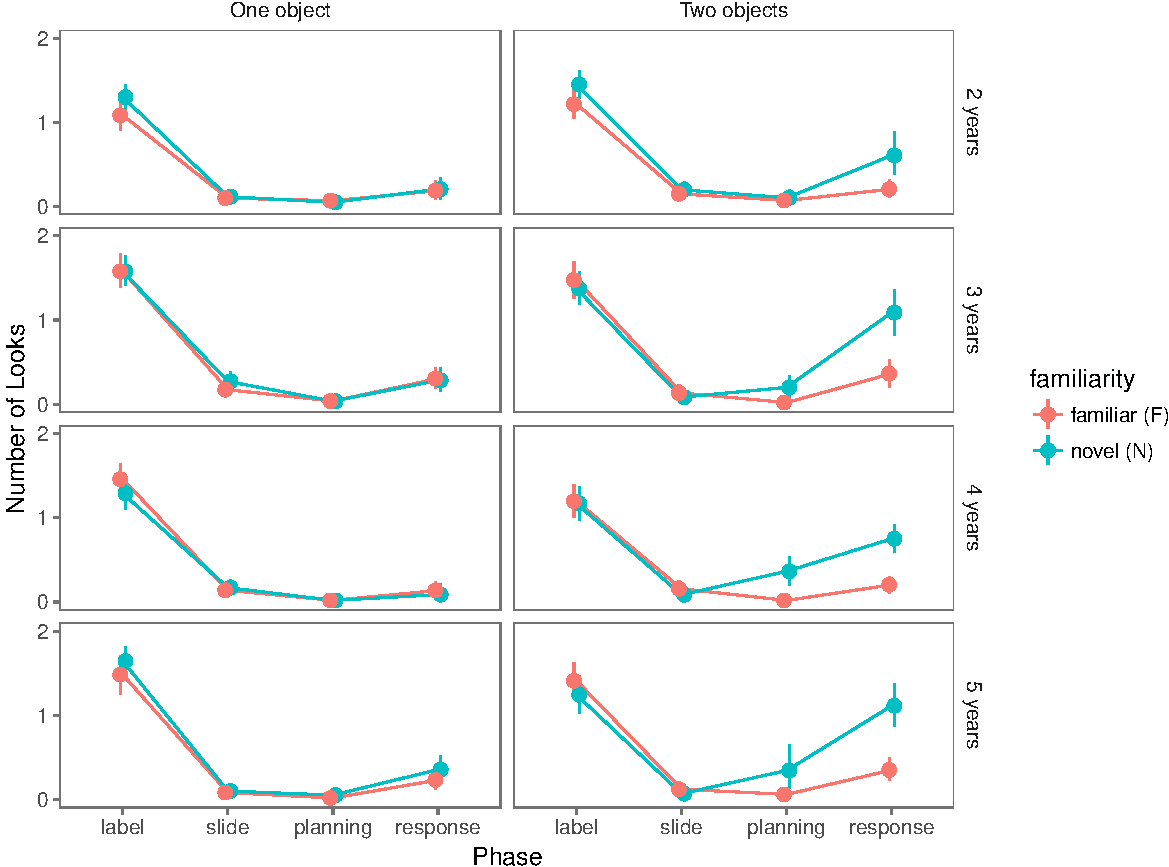
\includegraphics{figs/resultse1-1.pdf}
\caption{\label{fig:resultse1}Results of Experiment 1. Number of looks to
the experimenter based on phase, the number and familiarity of objects
present, and age. Age in months was entered as a continuous variable in
regression models but is presented here as a categorical variable for
visual simplicity. Error bars are 95 percent confidence intervals.}
\end{figure}

\begin{figure}
\centering
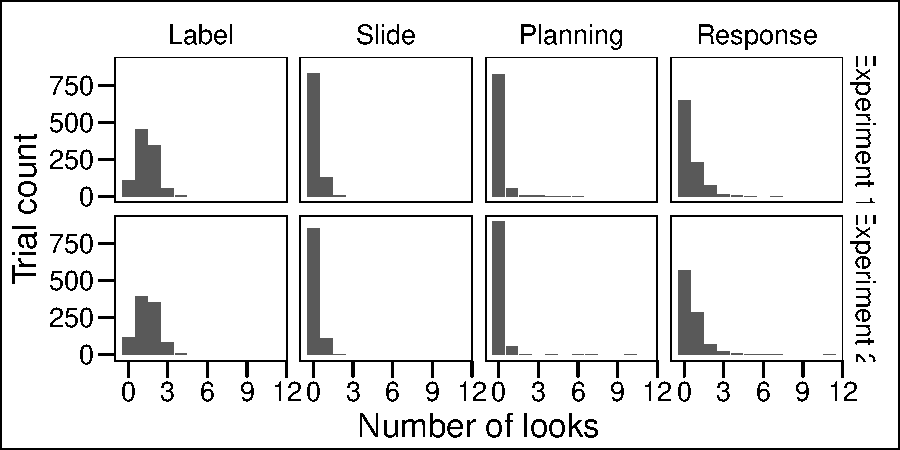
\includegraphics{figs/hist-1.pdf}
\caption{\label{fig:hist}Distribution of the number of looks to the speaker
in each phase.}
\end{figure}

\subsubsection{Social information gathering and referential
ambiguity}\label{social-information-gathering-and-referential-ambiguity}

We next examined children's looking behavior for each trial type across
the four phases of the trial. The distribution of number of looks are
presented in figure \ref{fig:resultse1}. Note that the most common
response is to reference the speaker at least once during the
\emph{label} phase, but to not reference the speaker at all during the
other phases. To test our prediction that referential ambiguity (i.e.,
having two novel objects) would produce more looking, we fit
mixed-effects linear regression models separately for each phase with
the following structure:
\texttt{number\ of\ looks\ \textasciitilde{}\ number\ of\ objects\ *\ familiarity\ *\ age\ in\ months\ +\ (number\ of\ objects\ +\ familiarity\ \textbar{}\ subject)}.
Our initial planned analysis, a single model with phase as a factor, did
not converge, and the model was subsequently trimmed according to our
standard laboratory analytic procedures.

We did not find any main or interaction effects of number of objects,
familiarity, or age on number of looks during the \emph{label} phase
(Figure \ref{fig:resultse1}). We also did not observe any significant
effects in the \emph{slide} phase. However, we found an interaction
effect of number of objects and familiarity during the \emph{planning}
(\(\beta\) = 0.21, \emph{p} \textless{} .001) and \emph{response} phases
(\(\beta\) = 0.60, \emph{p} \textless{} .001), such that NN trials were
associated with more looks. Age did not interact with number of objects
or familiarity.

An alternative analytic approach would be to fit a logistic
mixed-effects regression predicting \emph{whether or not} children look
to the speaker in each phase, rather than the number of times they do
so. In support of this approach, the distribution of looks is not normal
for the slide, planning, and response phases, with the majority of
trials containing no looks to the speaker (Figure \ref{fig:hist}). To
address this issue, we additionally fit separate logistic mixed-effects
regressions with the following structure:
\texttt{look\ (yes\ or\ no)\ \textasciitilde{}\ number\ of\ objects\ *\ familiarity\ *\ age\ in\ months\ +\ (number\ of\ objects\ +\ familiarity\ \textbar{}\ subject)}.
A single model with phase as a factor did not converge.

The results of these analyses were similar to those of the linear
models; number of objects and familiarity interacted in the
\emph{planning} and \emph{response} phases such that there was more
likely to be a look when there were two novel objects, (\(\beta\)s =
1.41, 1.90, \emph{p}s \textless{}.05 \& \textless{}.001). In addition,
there was a significant interaction of number and familiarity of objects
in the \emph{slide} phase, such that NN trials were less likely to be
associated with a look (\(\beta\) = -0.87, \emph{p} \textless{}.05).
This latter finding was not predicted, but could reflect children's
tendency to look more at novel stimuli, which would trade off with
looking at the speaker, particularly when there is no utility to looking
at the speaker, as when the objects are being slid across the table.

In summary, children looked to the speaker more often when planning and
executing a response under uncertainty. These results suggest that
children were aware that they did not have sufficient knowledge to
identify the referent and act on it, and referenced the speaker to
resolve this uncertainty. Surprisingly, we did not observe an effect of
age, suggesting that by age 2 children are already selective in their
information gathering to resolve lexical ambiguity.

Notably, and in contrast to Vaish et al., we did not find the expected
effect of referential ambiguity in the \emph{label} phase. Thus, mere
novelty or the presence of multiple objects was not enough to increase
children's looking when the experimenter was producing the label. Since
individuals tend to look at someone who is speaking, children may have
looked at the experimenter at least once regardless of lexical
ambiguity, minimizing possible condition differences. It is also
possible that children failed to predict that they would need more
information until later in the trial, when they were actually faced with
making a decision.

A third possibility is that this finding is an artifact of our design,
in which the speaker gazed at the center of the table rather than the
referent of the label. Children may have realized that the speaker's
gaze direction during labeling was not informative. Relatedly, children
may have found it strange to interact with a speaker who did not gaze at
the object they were labeling, which may have produced unnatural
patterns of looking. Experiment 2 tests these possibilities and further
examines whether children's information gathering is sensitive to graded
uncertainty.

\section{Experiment 2}\label{experiment-2}

Experiment 2 was designed to achieve several goals; first, we aimed to
replicate the finding from Experiment 1 that children reference a social
partner on the basis of referential ambiguity while executing a
decision. Second, we tested whether children's information gathering is
graded with respect to graded evidence about a label's referent.

To this end, we manipulated two sources of referential evidence. First,
we added trials with 1 novel and 1 familiar object (FN) and a novel
label. This condition contains evidence about reference since the
familiar item can be excluded (Markman \& Wachtel, 1988), but may not be
as conclusive as trials with a familiar target. Thus, we predicted that,
in the aggregate, children would show the most looking to the speaker in
the NN condition, the least in the FF condition, and an intermediate
amount in the FN condition.\\
Second, we manipulated between participants whether or not the speaker
gazed at the objects they referred to, and thus, whether or not their
gaze was an informative cue to reference. We predicted that having
access to referential gaze as an informative cue would make children
less likely to reference the speaker during their decision, but perhaps
more likely to reference the speaker during labeling. Critically, this
also allowed us to test whether children's information gathering is
selective on the basis of referential ambiguity during labeling if the
speaker's gaze is informative, addressing an interpretive issue in
Experiment 1.

Since we did not observe any difference between F and N trials in
Experiment 1, we eliminated single-object trials. Additionally, we
restricted the sample to 3- and 4-year-olds, as we did not observe
developmental differences in Experiment 1. Three- and 4-year-olds were
chosen because we planned to include age in months as a continuous
variable in our regression models, and contiguous age groups are thus
preferable. Furthermore, 2-year-olds seemed to have more difficulty
completing the task in Experiment 1, as evidenced by their lower
accuracy rate and higher rate of placing two objects in the bucket.

\subsection{Methods}\label{methods-1}

\subsubsection{Participants}\label{participants-1}

We recruited a planned sample of 80 children ages 3-4 years from the
Children's Discovery Museum in San Jose, California\footnote{Planned
  sample size, exclusion criteria, and analysis plan (including model
  specification) preregistered at \url{https://osf.io/y7mvt/}.}. The
sample included 40 3-year-olds (mean age 42.9 months) and 40 4-year-olds
(mean age 53.5 months). An additional 20 children participated but were
removed from analyses because they heard English less than 75\% of the
time at home (\emph{n} = 9), because they were unable to complete at
least half of the trials in the task (\emph{n} = 7), or due to
experimenter or technical errors (\emph{n} = 4).

\subsubsection{Stimuli and Design}\label{stimuli-and-design-1}

The stimuli and design were similar to Experiment 1 but included three
trial types: FF, NN, and FN. There were four of each trial type,
totaling twelve trials. In addition, we manipulated the experimenter's
gaze behavior between participants. For half of the participants, the
experimenter gazed at the center of the table while labeling objects
(uninformative gaze); for the remaining half, they gazed directly at the
objects they labeled (informative gaze).

\subsubsection{Procedure}\label{procedure-1}

The experimental and coding procedures were identical to Experiment 1,
except that there were three practice trials (two FF trials and one NN
trial). We chose this approach so that children could experience both
familiar and novel stimuli during practice, but would not be discouraged
by an overly difficult practice session. As in Experiment 1, children
were corrected if they chose the wrong object on FF trials but not NN
trials.

We again noted trials that should be excluded based on the same criteria
as in Experiment 1. We excluded 1.9\% of trials from 3-year-olds and no
trials from 4-year-olds. Inter-rater reliability for the number of looks
in each phase was again high, intraclass correlation \emph{r} = .97,
\emph{p} \textless{} .001. The mean durations of the phases for
Experiment 2 are presented in Table \ref{tab:phases}. They varied in
length according to the same pattern as in Experiment 1.

\subsection{Results and Discussion}\label{results-and-discussion-1}

\subsubsection{Accuracy}\label{accuracy-1}

\begin{figure}
\centering
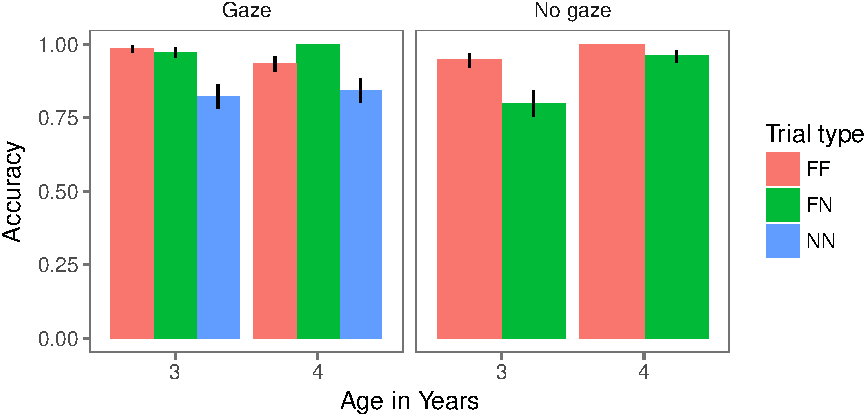
\includegraphics{figs/acce2-1.pdf}
\caption{\label{fig:acce2}Accuracy for trials with a correct answer
available (FF and FN, and all gaze trials) in Experiment 2. Error bars
are 95 percent confidence intervals.}
\end{figure}

Children's accuracy for trials with a correct answer possible (i.e., FF,
FN, and all trials with gaze) was calculated using the same criteria as
in Experiment 1 (Figure \ref{fig:acce2}). Children sometimes put two
items in the bucket, although they did so less frequently than in
Experiment 1, perhaps because there were two objects available on every
trial and it was thus less of a novelty (3-year-olds: 3.5\% of trials;
4-year-olds: 1.0\%). As in Experiment 1, the first item they placed in
the bucket was coded as their response. To quantify the effects of
familiarity, gaze, and age on accuracy, we fit the following
mixed-effects logistic regression model:
\texttt{correct\ \textasciitilde{}\ trial\ type\ *\ gaze\ +\ age\ in\ months\ +\ (1\textbar{}\ subject)}.
Accuracy was significantly lower for NN (\(\beta\) = -2.27, \emph{p}
\textless{} .001) and FN trials (\(\beta\) = -2.23, \emph{p} \textless{}
.001) compared to FF trials, and trial type interacted with gaze
condition such that accuracy was significantly higher in the gaze
condition for NN (\(\beta\) = 3.41, \emph{p} \textless{} .001) and FN
trials (\(\beta\) = 1.12, \emph{p} \textless{} .001). Age did not
significantly predict accuracy (\(\beta\) = 0.18, \emph{p} = .12).

\subsubsection{Information gathering and referential
ambiguity}\label{information-gathering-and-referential-ambiguity}

Experiment 2 was designed to test whether different amounts of
referential evidence elicit differential amounts of social information
gathering. If so, this would suggest that young children are sensitive
to graded evidence for a hypothesis (e.g., that this object is the
\enquote{blicket}). The amount of referential evidence was manipulated
through the familiarity of objects presented (NN vs FN vs FF trials) and
whether or not gaze was informative (gaze vs.~no gaze). If children are
sensitive to graded evidence, we might expect a pattern of looking that
conforms to (NN \textgreater{} FN \textgreater{} FF) and (no gaze
\textgreater{} gaze), with the possibility of an interaction between
gaze condition and familiarity.

Children's patterns of looking based on familiarity and gaze condition
are presented in Figure \ref{fig:resultse2}. To quantify the main and
interactive effects of familiarity, gaze condition, and age on
children's looking, we fit separate mixed-effects linear regression
models for each phase (label, planning, slide, response) with the
following structure:
\texttt{number\ of\ looks\ \textasciitilde{}\ familiarity\ *\ age\ in\ months\ *\ gaze\ +\ (1\ \textbar{}\ subject)}.

We found no effect of familiarity, gaze condition, or age on looking in
the \emph{label} phase. In the \emph{slide} phase, both FF (\(\beta\) =
0.09, \emph{p} \textless{} .01) and NN trials (\(\beta\) = 0.07,
\emph{p} = .047) elicited more looking compared to FN trials, and there
were no effects of or interactions with gaze condition or age. In the
\emph{planning} phase, we found that FF trials were associated with less
looking than FN trials (\(\beta\) = -0.11, \emph{p} = .045) and NN
trials were associated with more looking compared to FN trials
(\(\beta\) = 0.15, \emph{p} \textless{} .01), and there were no effects
of or interactions with gaze condition or age. In the \emph{response}
phase, FF trials elicited less looking (\(\beta\) = -0.43, \emph{p}
\textless{} .001) and NN trials elicited more looking (\(\beta\) = 0.22,
\emph{p} = .02) compared to FN trials. In addition, the gaze condition
was associated with less looking compared to the no-gaze condition
(\(\beta\) = -0.28, \emph{p} = .03), and gaze interacted with
familiarity such that FF trials in the gaze condition were associated
with more looking than FF trials in the no-gaze condition (\(\beta\) =
0.34, \emph{p} \textless{} .01).

As in Experiment 1, we additionally fit mixed-effects logistic
regressions with looking quantified as a binary variable (look vs.~no
look) for each phase, since the number of looks was not normally
distributed (Figure \ref{fig:histe1}). The models had the following
structure:
\texttt{look\ (yes\ or\ no)\ \textasciitilde{}\ trial\ type\ +\ age\ in\ months\ +\ (number\ of\ objects\ +\ familiarity\ \textbar{}\ subject)}.
The interaction terms between trial type and age were trimmed due to
model non-convergence. We observed a similar pattern of results compared
to the linear models, except that the difference between FF and FN
trials was not significant in the response phase. Additionally, similar
to Experiment 1, there was an effect of trial type in the \emph{slide}
phase such that children looked at the experimenter more for FF trials.

In summary, in the \emph{slide}, \emph{planning}, and \emph{response}
phases, children showed the pattern of responding with respect to graded
evidence that we predicted. They looked at the experimenter the most for
NN trials, the least for FF trials, and an intermediate amount for FN
trials. This suggests that the likelihood of children seeking
disambiguating information is tuned to the amount of referential
evidence they receive. Further supporting this idea, children looked
more at the experimenter when she did not gaze at the object she was
referring to during labeling, suggesting that children attended to this
evidence and it contributed to their certainty in their response.

Additionally, familiarity interacted with gaze condition, but not in the
predicted direction. Instead, FF trials with referential gaze elicited
more looking than FF trials without referential gaze. Although we did
not predict this result, it is possible that when children were already
quite certain, they were more likely to seek feedback from a social
partner whose gaze patterns were more naturalistic.

Finally, similar to Experiment 1, we did not observe selective looking
during the \emph{label} phase, even among children in the gaze
condition. This result rules out the possibility that children were less
selective during labeling during Experiment 1 because they learned that
the experimenter's gaze direction was not informative. Instead, young
children may attend to someone who is speaking regardless of the need
for disambiguation.

\begin{figure}
\centering
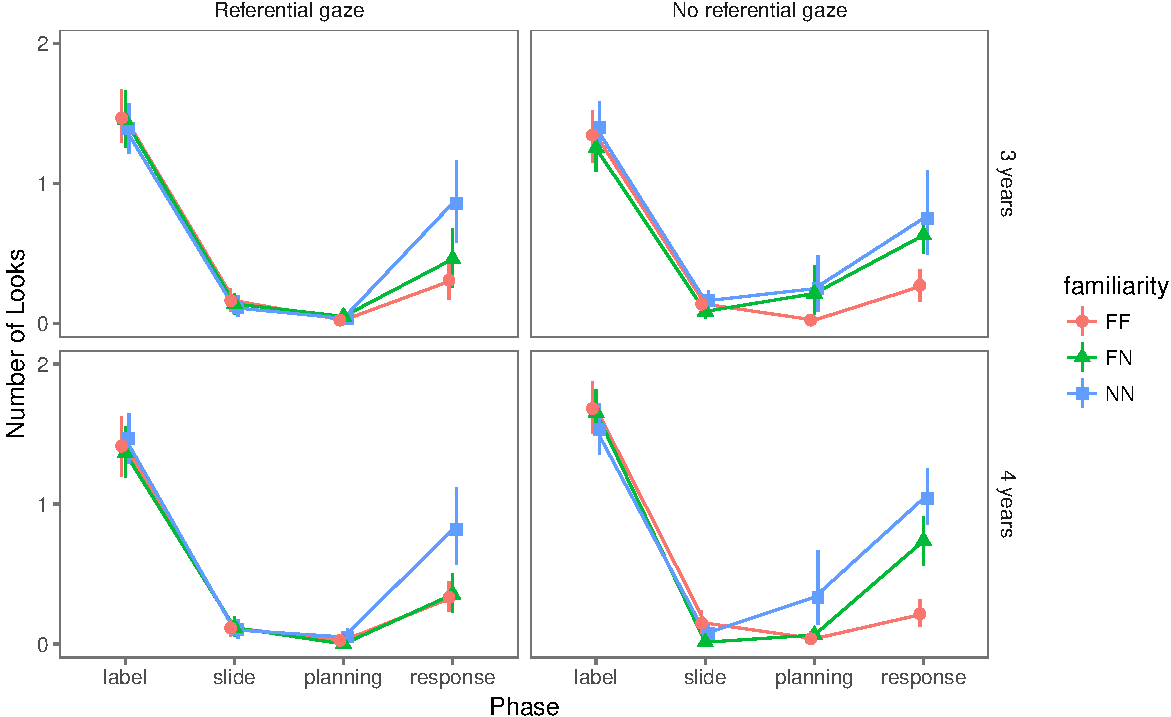
\includegraphics{figs/resultse2-1.pdf}
\caption{\label{fig:resultse2}Results of Experiment 2. Number of looks to
the experimenter based on phase, trial type, gaze condition, and age.
Age in months was entered as a continuous variable in regression models
but is presented here as a categorical variable for visual simplicity.
Error bars are 95 percent confidence intervals.}
\end{figure}

\section{General Discussion}\label{general-discussion}

During the preschool years, children are increasingly able to actively
gather information through help-seeking and exploration (Chouinard et
al., 2007; Schulz \& Bonawitz, 2007). They are also increasingly
proficient at explicitly identifying their gaps in knowledge and their
uncertainty in various domains (Coughlin et al., 2014; Hembacher \&
Ghetti, 2014; Lyons \& Ghetti, 2011; Rohwer et al., 2012). Do young
children similarly identify lexical ambiguity and engage in appropriate
active learning behaviors in response? Here, we examined whether young
children's social information gathering was associated with referential
uncertainty in situations in which the referent was either completely
novel or familiar (Experiment 1), and when there were differing amounts
of referential evidence (Experiment 2).

We found that referential ambiguity was strongly associated with
children's information gathering behavior. Specifically, we observed
this selectivity when children were planning and executing their
decision. We speculate that children referenced the speaker during the
decision process because they expected evaluative feedback about their
demonstrated choice, either implicitly through the adult's facial
expressions, or through an explicit response. This idea is consistent
with other recent findings that preschoolers and toddlers seek help
selectively when a problem is difficult or they are less skilled (Goupil
et al., 2016; Vredenburgh \& Kushnir, 2015).

We also found that children's information-seeking reflected graded
referential evidence. In the case of FN trials, children could solve the
problem of reference by excluding the familiar item (Markman \& Wachtel,
1988; Merriman, Bowman, \& MacWhinney, 1989), and indeed, they chose the
correct object most of the time for these trials. If children simply
monitored the presence or absence of such cues, they would have
consistently responded to FN trials with certainty. Instead, they sought
information in a graded fashion, looking at the experimenter less than
for NN trials but more than for FF trials. Overall, they also exhibited
less looking when referential gaze was present than when it was not.
Intriguingly, children appear to remain uncertain when their only cue to
reference is the adult's gaze during labeling --- there was no
difference between NN trials with and without gaze. This finding
suggests that referential gaze may be a weaker cue compared to ruling
out a familiar object.

These findings are important given that the ability to monitor the
likelihood of accuracy based on graded evidence is assumed important for
decision-making and behavioral regulation across development (Krebs \&
Roebers, 2010; Yeung \& Summerfield, 2012). Being able to monitor graded
epistemic uncertainty allows individuals to gate out information that
does not meet a criterion level of certainty based on individual goals
or task demands (Koriat \& Goldsmith, 1996). The current findings are
consistent with the possibility that preschoolers engage in this type of
reasoning, given that their uncertainty tracked quantitatively with the
amount of evidence available.

On the other hand, we found no evidence for selective information
gathering while the speaker was producing the label. One possibility is
that young children do not recognize the need for disambiguating
information until they need to make a decision (Markman, 1977). Another
possibility is that children spontaneously look at a speaker regardless
of ambiguity, and additional looking was not necessary. This latter
possibility seems more credible, given that children typically looked at
the speaker at least once during labeling. Notably, Vaish et al.
observed selective referencing during labeling among infants. Since
infants in that study were holding one of the objects during labeling,
referencing the speaker would have required them to disengage from that
object, and may therefore have been more costly, promoting selectivity.
Future research with preschool-aged children that includes a greater
trade-off between attentional options would help to distinguish among
these possibilities.

Contrary to our expectations, we did not observe developmental
differences in children's information seeking. We sampled a broad age
range (2 to 5 years) due to previous evidence for improvements in
metacognitive performance during the preschool years (Coughlin et al.,
2014; Hembacher \& Ghetti, 2014; Lyons \& Ghetti, 2011; Rohwer et al.,
2012). However, we found that 2-year-olds were equally likely to be
selective in their information seeking compared to 5-year-olds. There
are several possible explanations for this finding. On the one hand, it
could be that children's monitoring of lexical ambiguity and ability to
selectively seek out disambiguating evidence are both firmly in place by
age 2, and do not develop in the following years. Indeed, there is
evidence from Vaish et al. that infants ages 13 and 18 months
selectively reference a speaker's gaze direction when her referent is
ambiguous, suggesting that sensitivity to lexical uncertainty develops
early. Typically-developing children acquire a substantial vocabulary by
age 2, so if lexical uncertainty monitoring is important for language
acquisition, it may not be surprising that 2-year-olds demonstrate this
ability.

Another possibility is that children's awareness of uncertainty (in the
linguistic domain and beyond) becomes more concrete throughout early
childhood, but that information-seeking is a particularly sensitive
measure of early uncertainty monitoring compared to explicit report (see
Kloo et al. for a similar argument). Developmental differences in
information-seeking during early childhood could be minimal because they
do not rely as strongly on later-developing metacognitive processes and
verbal ability.

In line with this idea, the behavior we examined here, selective social
information-gathering, could fall into a spectrum of active learning
behaviors beginning in infancy. Infants direct their attention to
salient aspects of the environment that are most likely to yield
information, including faces and hands. As infants learn to locomote,
first by crawling and then by walking, they have access to a broader set
of information sources. As children learn to speak and to manipulate
objects in the environment, they have more opportunity still to seek out
information to disambiguate areas of uncertainty. These physical and
cognitive developmental trajectories may procede in parallel to
metacognitive advancements that allow children to more acutely identify
gaps in knowlege that they can then seek to fill. From this perspective,
the present investigation illustrates one piece in the puzzle of
children's developing contributions to their own learning.

There are limitations to the current investigation. First, although we
assume that children hoped to glean disambiguating information from the
adult experimenter when they visually referenced her, we do not know
what type of evidence evidence they expected to receive (e.g., direct
help, informative gaze, or an affective response). This is especially
relevant as children of different ages, despite showing the same
patterns of looking, might have had distinct expectations about the type
of information or help they would receive. Additionally, in Experiment
1, children sometimes ignored the instruction to place only one item in
the bucket, particularly 2-year-olds. Although we speculate that younger
children showed this behavior because they found it entertaining to
place both objects in the bucket, this behavior could also reflect a
different understanding or approach to the task compared to older
children. Future research should attempt to measure
information-gathering behavior in a range of tasks that equate for
difficult across ages.

Overall, these results provide further evidence that preschool-aged
children monitor graded uncertainty in their mental representations
generally, and in lexical ambiguity specifically. Furthermore, they act
on that uncertainty through spontaneous information-seeking. These
behaviors may in part underlie the rapid acquisition of language during
early childhood.

\section{Acknowledgements}\label{acknowledgements}

We thank Veronica Cristiano for assisting with data collection. EH was
supported by a generous gift from Kinedu SAPI de CV.

\section{References}\label{references}

\setlength{\parindent}{-0.1in} \setlength{\leftskip}{0.125in} \noindent

\hypertarget{refs}{}
\hypertarget{ref-Baayen2008}{}
Baayen, R. H., Davidson, D. J., \& Bates, D. M. (2008). Mixed-effects
modeling with crossed random effects for subjects and items.
\emph{Journal of Memory and Language}, \emph{59}(4), 390--412.

\hypertarget{ref-Balcomb2008}{}
Balcomb, F. K., \& Gerken, L. (2008). Three-year-old children can access
their own memory to guide responses on a visual matching task.
\emph{Developmental Science}, \emph{11}(5), 750--760.

\hypertarget{ref-Barr2013}{}
Barr, D. J., Levy, R., Scheepers, C., \& Tily, H. J. (2013). Random
effects structure for confirmatory hypothesis testing: Keep it maximal.
\emph{Journal of Memory and Language}, \emph{68}(3), 255--278.

\hypertarget{ref-Bonawitz2014}{}
Bonawitz, E., Denison, S., Gopnik, A., \& Griffiths, T. L. (2014).
Win-Stay, Lose-Sample: A simple sequential algorithm for approximating
Bayesian inference. \emph{Cognitive Psychology}, \emph{74}(C), 35--65.

\hypertarget{ref-Call2001}{}
Call, J., \& Carpenter, M. (2001). Do apes and children know what they
have seen? \emph{Animal Cognition}, \emph{3}(4), 207--220.

\hypertarget{ref-Chouinard2007}{}
Chouinard, M. M., Harris, P. L., \& Maratsos, M. P. (2007). Children's
questions: A mechanism for cognitive development. \emph{Monographs of
the Society for Research in Child Development}, \emph{72}, 1--129.

\hypertarget{ref-Coughlin2014}{}
Coughlin, C., Hembacher, E., Lyons, K. E., \& Ghetti, S. (2014).
Introspection on uncertainty and judicious help-seeking during the
preschool years. \emph{Developmental Science}, \emph{18}(6), 957--971.

\hypertarget{ref-Frank2016}{}
Frank, M. C., Braginsky, M., Yurovsky, D., \& Marchman, V. A. (2016).
Wordbank: an open repository for developmental vocabulary data.
\emph{Journal of Child Language}, \emph{44}(03), 677--694.

\hypertarget{ref-Ghetti2013}{}
Ghetti, S., Hembacher, E., \& Coughlin, C. (2013). Feeling Uncertain and
Acting on It During the Preschool Years: A Metacognitive Approach.
\emph{Child Development Perspectives}, \emph{7}(3), 160--165.

\hypertarget{ref-Goupil2016}{}
Goupil, L., Romand-Monnier, M., \& Kouider, S. (2016). Infants ask for
help when they know they dont know. \emph{Proceedings of the National
Academy of Sciences}, \emph{113}(13), 3492--3496.

\hypertarget{ref-Hembacher2014}{}
Hembacher, E., \& Ghetti, S. (2014). Dont look at my answer: Subjective
uncertainty underlies preschoolers exclusion of their least accurate
memories. \emph{Psychological Science}, \emph{25}(9),
0956797614542273--1776.

\hypertarget{ref-Kidd2012}{}
Kidd, C., Piantadosi, S. T., \& Aslin, R. N. (2012). The Goldilocks
Effect: Human Infants Allocate Attention to Visual Sequences That Are
Neither Too Simple Nor Too Complex. \emph{PLoS ONE}, \emph{7}(5),
e36399--8.

\hypertarget{ref-Kidd2014}{}
Kidd, C., Piantadosi, S. T., \& Aslin, R. N. (2014). The Goldilocks
Effect in Infant Auditory Attention. \emph{Child Development},
\emph{19}, n/a--n/a.

\hypertarget{ref-Koriat1996}{}
Koriat, A., \& Goldsmith, M. (1996). Monitoring and control processes in
the strategic regulation of memory accuracy. \emph{Psychological
Review}, \emph{103}(3), 490--517.

\hypertarget{ref-Krebs2010}{}
Krebs, S. S., \& Roebers, C. M. (2010). Children's strategic regulation,
metacognitive monitoring, and control processes during test taking.
\emph{British Journal of Educational Psychology}, \emph{80}(3),
325--340.

\hypertarget{ref-Lyons2011a}{}
Lyons, K. E., \& Ghetti, S. (2011). The development of uncertainty
monitoring in early childhood. \emph{Child Development}, \emph{82}(6),
1778--1787.

\hypertarget{ref-Lyons2011}{}
Lyons, K. E., \& Zelazo, P. D. (2011). Monitoring, metacognition, and
executive function: Elucidating the role of self-reflection in the
development of self-regulation. \emph{Advances in Child Development and
Behavior}, \emph{40}, 379--412.

\hypertarget{ref-Marazita2004}{}
Marazita, J. M., \& Merriman, W. E. (2004). Young childrens judgment of
whether they know names for objects: The metalinguistic ability it
reflects and the processes it involves. \emph{Journal of Memory and
Language}, \emph{51}(3), 458--472.

\hypertarget{ref-Markant2016}{}
Markant, D. B., Ruggeri, A., Gureckis, T. M., \& Xu, F. (2016). Enhanced
Memory as a Common Effect of Active Learning. \emph{Mind, Brain, and
Education}, \emph{10}(3), 142--152.

\hypertarget{ref-Markman1977}{}
Markman, E. M. (1977). Realizing that you don't understand: A
preliminary investigation. \emph{Child Development}, \emph{48}(3),
986--992.

\hypertarget{ref-Markman1988}{}
Markman, E. M., \& Wachtel, G. F. (1988). Children's use of mutual
exclusivity to constrain the meanings of words. \emph{Cognitive
Psychology}, \emph{20}, 121--157.

\hypertarget{ref-Merriman1989}{}
Merriman, W. E., Bowman, L. L., \& MacWhinney, B. (1989). The mutual
exclusivity bias in children's word learning. \emph{Monographs of the
Society for Research in Child Development}, \emph{54},
i--iii--v--1--129.

\hypertarget{ref-Rohwer2012}{}
Rohwer, M., Kloo, D., \& Perner, J. (2012). Escape From Metaignorance:
How Children Develop an Understanding of Their Own Lack of Knowledge.
\emph{Child Development}, \emph{83}(6), 1869--1883.

\hypertarget{ref-Ruggeri2017}{}
Ruggeri, A., Sim, Z. L., \& Xu, F. (2017). ``Why is Toma late to school
again?'' Preschoolers identify the most informative questions.
\emph{Developmental Science}.

\hypertarget{ref-Schulz2007}{}
Schulz, L. E., \& Bonawitz, E. (2007). Serious fun: Preschoolers engage
in more exploratory play when evidence is confounded.
\emph{Developmental Psychology}, \emph{43}(4), 1045--1050.

\hypertarget{ref-Teglas2011}{}
Teglas, E., Vul, E., Girotto, V., Gonzalez, M., Tenenbaum, J. B., \&
Bonatti, L. L. (2011). Pure Reasoning in 12-Month-Old Infants as
Probabilistic Inference. \emph{Science}, \emph{332}(6033), 1054--1059.

\hypertarget{ref-Vaish2011}{}
Vaish, A., Demir, Ö. E., \& Baldwin, D. (2011). Thirteen- and
18-month-old infants recognize when they need referential information.
\emph{Social Development}, \emph{20}(3), 431--449.

\hypertarget{ref-Vredenburgh2015}{}
Vredenburgh, C., \& Kushnir, T. (2015). Young children's help-seeking as
active information gathering. \emph{Cognitive Science}, \emph{40}(3),
697--722.

\hypertarget{ref-Xu2013}{}
Xu, F., \& Kushnir, T. (2013). Infants are rational constructivist
learners. \emph{Current Directions in Psychological Science},
\emph{22}(1), 28--32.

\hypertarget{ref-Yeung2012}{}
Yeung, N., \& Summerfield, C. (2012). Metacognition in human
decision-making: confidence and error monitoring. \emph{Philosophical
Transactions of the Royal Society B: Biological Sciences},
\emph{367}(1594), 1310--1321.






\end{document}
